
\documentclass{article}
\usepackage[utf8]{inputenc}
\usepackage{graphicx}
%% -----------------------------
%% TITLE
%% -----------------------------
\title{Homework \#3 Solution} %% Assignment Title

\author{Anju Kumari\\ %% Student name
COMS 665A -  Advanced Topics in Software Engineering: Foundations\\ %% Code and course name
\textsc{Iowa State University}
}
\date{}

\begin{document}

\maketitle

{\bf Algorithm to convert Task Precedence Graph into a  Petri net} \\
-------------------------------------------------------------------\\

Step 1:  If there is edge from place1 to place2 then create a transition t1  between place1 and place2. \\
Step 2: Create a input arc from place1 to t1 and an output arc from t1 to place2.\\
Step 3: If there are more than one children of a task then create output arc from its transion to children.  \\
Step 4: If more than one tasks are merging into single task then create a single transition for all these tasks. \\
Step 5: Input arc originates from a place and ends at a transition function. \\
Step 6: Output arc can be distributed among the source node's children. \\
Step 7: Initialize source node. \\
Step 8: Run in Smart.


\begin{figure}[h]
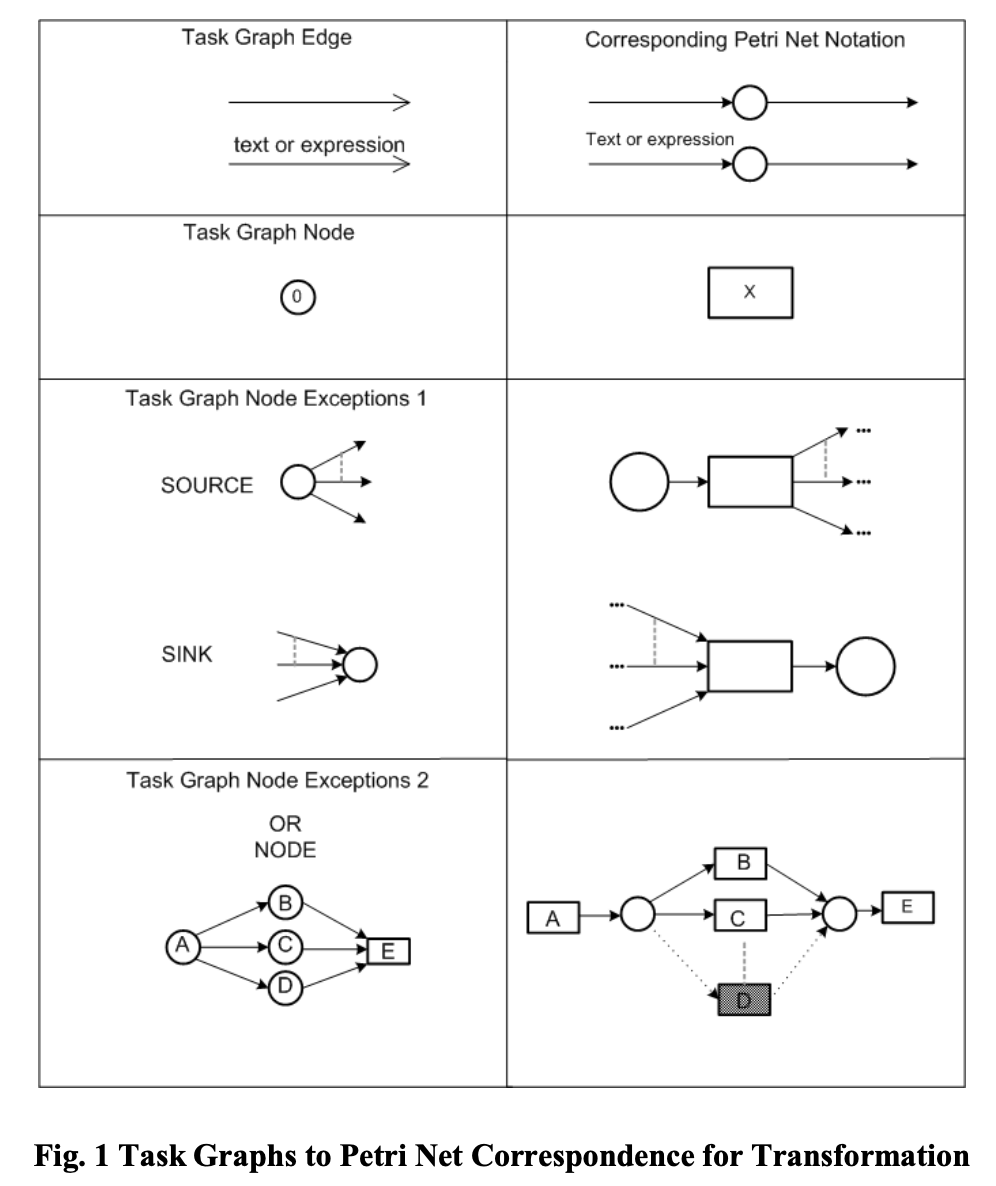
\includegraphics[width=10cm]{pn}
\end{figure}


 

\end{document}

